\subsection{Построение сетевого графика} \label{net_graph}

Для определения временных затрат и трудоемкости разработки ПО используем метод сетевого планирования. Метод сетевого планирования позволяет установить единой схемой связь между всеми работами в виде наглядного и удобного для восприятия изображения (сетевого графика), представляющего собой информационно-динамическую модель, позволяющую определить продолжительность и трудоёмкость, как отдельных этапов, так и всего комплекса работ в целом.

\vspace{\baselineskip}
Составление сетевой модели включает в себя оценку степени детализации комплекса работ и определения логической связи между отдельными работами.
С этой целью составляется перечень всех основных событий и работ. В перечне указываются кодовые номера событий, наименования событий в последовательности от исходного к завершающему, кодовые номера работ, перечень всех работ, причём подряд указываются все работы, которые начинаются после наступления данного события.

\vspace{\baselineskip}
Основные события и работы проекта представлены в таблице \ref{table:events}.


\begin{center}
\renewcommand\multirowsetup{\centering}
\begin{longtable}[h]{| >{\centering}m{1cm} | >{\centering}m{4cm} | >{\centering}m{1.5cm} | >{\centering}m{5cm} | >{\centering}m{1cm} | >{\centering}m{1cm} |}
  \captionsetup{justification=raggedright}
	\caption{Основные события и работы проекта} \label{table:events} \tabularnewline
  \hline


\rowcolor{Gray}   $N_i$  &   Наименование события &  Код работы &   Работа &   $t$, чел / час &   $t$,  чел / день \tabularnewline \hline \endfirsthead   \hline
 \multicolumn{6}{|c|}{\small\slshape (продолжение таблицы \ref{table:events})}        \tabularnewline \hline
 \rowcolor{Gray}   $N_i$  &   Наименование события &   Код работы &    Работа &  $t$, чел / час &  $t$,  чел / день               \tabularnewline \hline
                                              \endhead        \hline
 % \multicolumn{6}{|r|}{\small\slshape продолжение следует}  \tabularnewline \hline
                                              \endfoot        \hline
                                              \endlastfoot


 % \rowcolor{Gray}  $N_i$  &  Наименование события &  Код работы &   Работы &  $t$, чел / час &  $t$,  чел / день \tabularnewline \hline

 0 & Разработка ПО начата & 0-1 & Получение задания, анализ полученных требований к разрабатываемому ПО & 8 & 1 \tabularnewline \hline

 1 & Анализ полученных требований к разрабатываемому ПО проведен & 1-2 & Разработка и утверждение ТЗ & 24 & 3 \tabularnewline \hline
 
 2 & ТЗ разработано и утверждено & 2-3 & Анализ предметной области и существующих решений & 32 & 4 \tabularnewline \hline
 
 3 & Анализ предметной области и существующих решений проведён & 3-4 & Анализ потоков данных в процессе электронного документооборота & 80 & 10 \tabularnewline \hline
 
 4 & Анализ потоков данных в процессе электронного документооборота проведён & 4-5 & Разработка общей структуры ПО и пользовательского интерфейса & 32 & 4 \tabularnewline \hline
 
 5 & Разработка общей структуры ПО и пользовательского интерфейса завершена & 5-6 & Разработка алгоритмов, структуры входных и выходных данных & 72 & 9 \tabularnewline \hline %\pagebreak
 
\multirow{2}{1cm}{6} & \multirow{2}{4cm}{Разработка алгоритмов, структуры входных и выходных данных завершена} & 6-7 & Реализация пользовательского интерфейса & 40 & 5 \tabularnewline \cline{3-6}
& & 6-8 & Программная реализация модулей защищенной обработки, передачи и хранения информации & 80 & 10 \tabularnewline \hline

7 & Реализация пользовательского интерфейса завершена & 7-8 & Фиктивная работа & 0 & 0 \tabularnewline \hline

\multirow{6}{1cm}{8} & \multirow{6}{4cm}{Программная реализация модулей защищенной обработки, передачи и хранения информации завершена} & & & & \tabularnewline
 & & & & & \tabularnewline
 & & 8-9 & Тестирование ПО & 64 & 8 \tabularnewline 
 & & & & & \tabularnewline
 & & & & & \tabularnewline \cline{3-6} 
 & & & & & \tabularnewline
 & & 8-10 & Разработка документации & 80 & 10 \tabularnewline
 & & & & & \tabularnewline \hline

 9 & Тестирование ПО завершено & 9-11 & Внесение изменений в ПО & 40 & 5 \tabularnewline \hline

 10 & Документация разработана & 1-12 & Фиктивная работа & 0 & 0 \tabularnewline \hline

 11 & Внесение изменений в ПО закончено & 11-12 & Фиктивная работа & 0 & 0 \tabularnewline \hline

 12 & Разработка ПО закончена & --- & --- & --- & --- \tabularnewline \hline
\end{longtable}
\end{center}


Рассчитанные оставшиеся параметры элементов сети (сроки наступления событий, резервы времени событий, полный и свободный резервы времени работ) приведены в таблице \ref{table:time_per_work}.
\begin{table} [h!]
  
  \captionsetup{justification=raggedright}
  \caption{Временные затраты на каждый этап работы}\label{table:time_per_work}
 \begin{center}
  \begin{tabular}{| c | >{\centering}m{1.5cm} | >{\centering}m{1.5cm} | >{\centering}m{1.5cm} | >{\centering}m{1.5cm} | >{\centering}m{1.5cm} | >{\centering}m{1.5cm} | >{\centering}m{1.5cm} |}
  \hline
 \rowcolor{Gray} $N_i$  & Код работы $i-j$ & $t_{i-j}$, чел / день &  $T_i^P$, чел / день & $T_i^\textrm{П}$, чел / день & $R_i$, чел / день & $R_{i-j}^\textrm{П}$, чел / день & $R_{i-j}^C$, чел / день \tabularnewline \hline

 0 & 0-1 & 1 & 0 & 0 & 0 & 0 & 0 \tabularnewline \hline
 1 & 1-2 & 3 & 1 & 1 & 0 & 0 & 0 \tabularnewline \hline
 2 & 2-3 & 4 & 4 & 4 & 0 & 0 & 0 \tabularnewline \hline
 3 & 3-4 & 10 & 8 & 8 & 0 & 0 & 0 \tabularnewline \hline
 4 & 4-5 & 4 & 18 & 18 & 0 & 0 & 0 \tabularnewline \hline
 5 & 5-6 & 9 & 22 & 22 & 0 & 0 & 0 \tabularnewline \hline
 \multirow{2}{*}{6} & 6-7 & 5 & \multirow{2}{*}{31} & \multirow{2}{*}{31} & \multirow{2}{*}{0} & 5 & 0 \tabularnewline \cline{2-3} \cline{7-8}
  & 6-8 & 10 & & & & 0 & 0 \tabularnewline \hline
  7 & 7-8 & 0 & 36 & 41 & 5 & 0 & 0 \tabularnewline \hline
\multirow{2}{*}{8} & 8-9 & 8 & \multirow{2}{*}{41} & \multirow{2}{*}{41} & \multirow{2}{*}{0} & 0 & 0 \tabularnewline \cline{2-3} \cline{7-8}
  & 8-10 & 10 & & & & 3 & 0 \tabularnewline \hline
  9 & 9-11 & 5 & 49 & 49 & 0 & 0 & 0 \tabularnewline \hline
  10 & 10-12& 0 & 51 & 54 & 3 & 0 & 0 \tabularnewline \hline
  11 & 11-12 & 0 & 54 & 54 & 0 & 0 & 0 \tabularnewline \hline
  12 & - & - & 54 & 54 & 0 & 0 & 0 \tabularnewline \hline
   \end{tabular}
 \end{center}
\end{table}

Здесь \textbf{ранний срок совершения события} $T_j^P$ определяет минимальное время, необходимое для выполнения всех работ, предшествующих данному событию и равен продолжительности наибольшего из путей, ведущих от исходного события к рассматриваемому:
\begin{equation}
  \label{eq:T_j^P}
T_j^P = max \{ T_i^P + t_{i-j}\}.
\end{equation}

\textbf{Поздний срок совершения события} $T_i^\textrm{П}$ – это максимально допустимое время наступления данного события, при котором сохраняется возможность соблюдения ранних сроков наступления последующих событий. Поздние сроки равны разности между поздним сроком совершения $j$-го события и продолжительностью работы $i-j$:
\begin{equation}
  \label{eq:T_j_late}
T_i^\textrm{П} = min \{ T_j^\textrm{П} - t_{i-j}\}.
\end{equation}

\textbf{Критический путь} – это максимальный путь от исходного события до завершения проекта. Его определение позволяет обратить внимание на перечень событий, совокупность которых имеет нулевой резерв времени.

Все события в сети, не принадлежащие критическому пути, имеют \textbf{резерв времени} $R_i$,  показывающий, на какой предельный срок можно задержать наступление этого события, не увеличивая сроки окончания работ:
\begin{equation}
  \label{eq:R_i}
R_i = T_i^\textrm{П} - T_i^P.
\end{equation}

\textbf{Полный резерв времени работы} $R_{i-j}^\textrm{П}$ и \textbf{свободный резерв времени} $R_{i-j}^C$ работы можно определить, используя следующие соотношения:
\begin{equation}
  \label{eq:R_ij_full}
R_{i-j}^\textrm{П} = T_j^\textrm{П} - T_i^P - t_{i-j}.
\end{equation}
\begin{equation}
  \label{eq:R_ij^C}
R_{i-j}^C = T_j^P - T_i^P - t_{i-j}.
\end{equation}

Полный резерв работы показывает максимальное время, на которое можно увеличить длительность работы или отсрочить ее начало, чтобы не нарушился срок завершения проекта в целом. Свободный резерв работы показывает максимальное время, на которое можно увеличить продолжительность работы или отсрочить ее начало, не меняя ранних сроков начала последующих работ.

Сетевой график приведён на рис. \ref{img:net_graph}.

\begin{figure} [h] 
  \center
  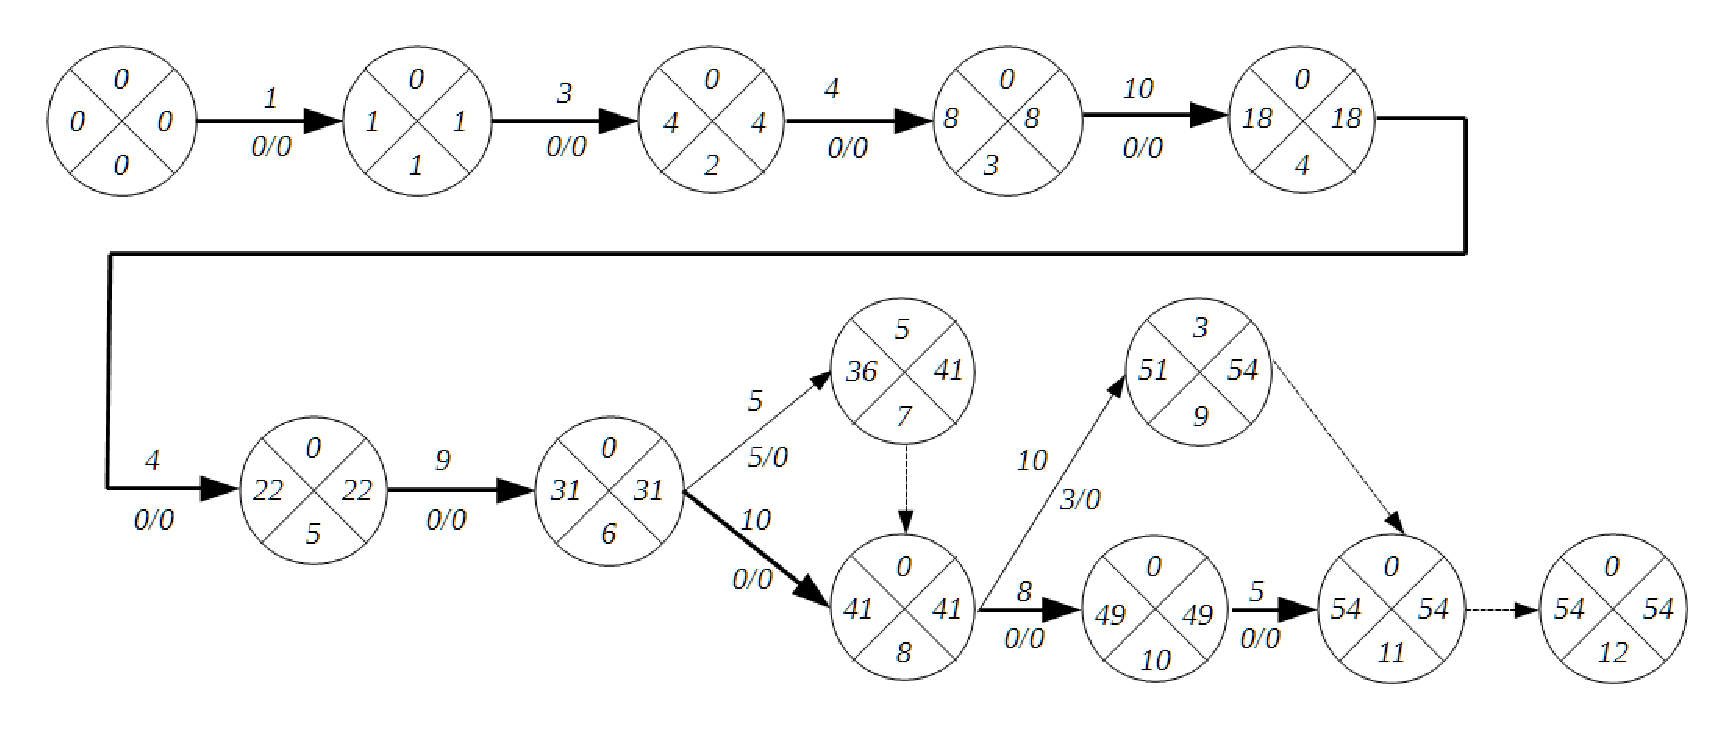
\includegraphics [scale=0.6] {netgraph}
  \caption{Сетевой график выполнения работ} 
  \label{img:net_graph}  
\end{figure}